\documentclass{standalone}
\usepackage{tikz}
\usepackage{siunitx} % Para la notación de unidades

\begin{document}

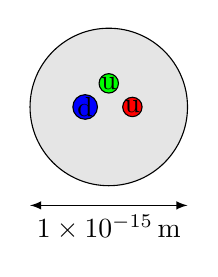
\begin{tikzpicture}
    % Radio del protón
    \def\R{1} % Radio de 1 cm (diámetro 2 cm)
    
    % Círculo del protón
    \node[circle, draw, fill=gray!20, minimum size=2cm, inner sep=0pt] {};
    
    % Posiciones de los quarks
    \node[circle, draw, fill=red, minimum size=0.15cm, inner sep=0pt] at ({\R*0.3}, {0}) {u};
    \node[circle, draw, fill=blue, minimum size=0.15cm, inner sep=0pt] at ({-\R*0.3}, {0}) {d};
    \node[circle, draw, fill=green, minimum size=0.15cm, inner sep=0pt] at ({0}, {\R*0.3}) {u};
    
    % Escala
    \draw[latex-latex] (-1,-1.25)--(1,-1.25);
    \node[below] at (0,-1.25){\SI{1e-15}{m}};
\end{tikzpicture}

\end{document}
